\chapter{Objektorientierte Programmierung}
Das objektorientierte Programmierparadigma ist das aktuell, gerade in der Anwendungsentwicklung, am häufigsten eingesetzte Programmierparadigma.

\begin{quote}
\enquote{
Mittlerweile ist Objektorientierung so populär geworden, dass sich viele Software-Produkte, Werkzeuge und Vorgehensmodelle schon aus Marketing-Gründen objektorientiert nennen – unnötig zu sagen, dass nicht überall, wo ”objektorientiert“ draufsteht, auch ”objektorientiert“ drin ist.} 
\cite[S.16]{PoetzschHeffter.2009}
\end{quote}

Doch welche Merkmale müssen auf eine Programmiersprache zutreffen, um sie objektorientierte Programmiersprache nennen zu können?
Laut \cite{Lahres.2011} gelten folgende Grundelemente als Basis einer objektorientierten Programmiersprache:

\begin{itemize}
    \item Vererbung
    \item Datenkapselung
    \item Polymorphie
\end{itemize}

Erfüllen Go und Swift die Grundvoraussetzungen einer objektorientierten Programmiersprache? Dies soll in diesem Kapitel erörtert werden.

\section{Vererbung}
Ein zentrales Element der Objektorientierten Programmierung ist die Vererbung. 
Laut \cite[S. 145]{PoetzschHeffter.2009} bedeutet Vererbung im engeren Sinne, dass eine Klasse Programmteile von einer anderen Klasse automatisch übernimmt. 
Bei der einfachen Form der Vererbung, auch Einfachvererbung genannt, erbt die Klasse von genau einer anderen Klasse.
Eine andere Form der Vererbung ist die sogenannte Mehrfachvererbung. 
Bei der Mehrfachvererbung kann eine Klasse von mehreren Klassen erben.
Von \cite[S.41]{Oestereich.1999} wird darauf hingewiesen, dass zur Vererbung  verschiedene Alternativen existieren und die Möglichkeiten und die Sinnhaftigkeit von Vererbung häufig überschätzt werden.


Dieser Abschnitt beschäftigt sich mit der Frage ob Go und Swift Vererbung unterstützen, beziehungsweise, ob eine Aufgabe alternativ implementiert werden kann.
Zu diesem Zweck wird eine gegebene Vererbungshierarchie in Form eines UML-Klassendiagramms beispielhaft in Go und Swift implementiert. 
Das folgende Beispiel orientiert sich an \cite[]{WilliamKennedy.2013}.

\begin{figure}[H]
    \centering
    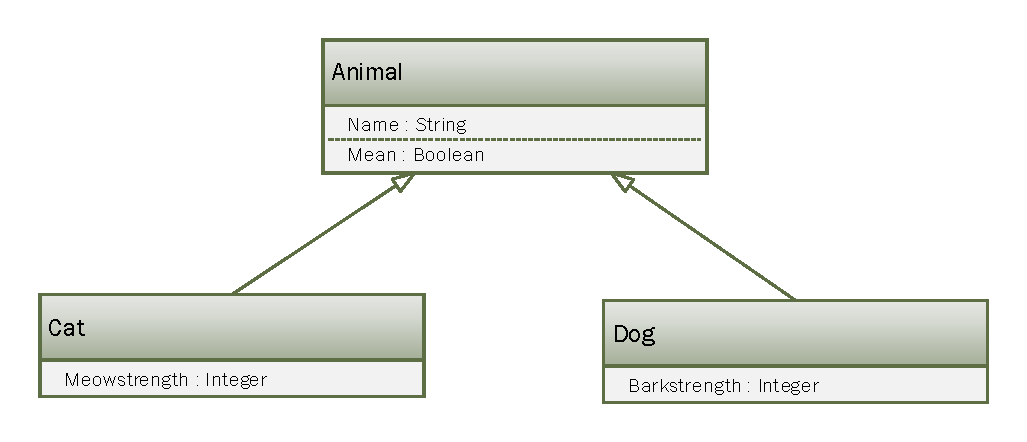
\includegraphics[width=\textwidth]{Images/Klassendiagramm.pdf}
    \caption{Klassendiagramm}
    \label{fig:Klassendiagramm}
\end{figure}

\autoref{fig:Klassendiagramm} zeigt ein UML-Klassendiagramm mit einer einfachen Vererbungs-Hierarchie.
Die beiden Klassen \emph{Cat} und \emph{Dog} erben die Eigenschaften der Klasse \emph{Animal}.


Da Go keine Vererbung beherrscht, ist Komposition\todo{Glossar} die einzige Möglichkeit eine Hierarchie abzubilden \cite[]{Kennedy.2016}.
Das \autoref{lst:VererbungGo} zeigt die Implementierung der Vererbungshierarchie aus \autoref{fig:Klassendiagramm}.

\begin{listing}[H]
\caption{Vererbung in Go \cite{Kennedy.2016}}
\label{lst:VererbungGo}
\begin{GoCode}
type Animal struct {
    Name string
    mean bool
}

type Cat struct {
    Basics Animal
    MeowStrength int
}

type Dog struct {
    Animal
    BarkStrength int
}
\end{GoCode}
\end{listing}

In Zeile 1-4 wird eine neue struct \emph{Animal} definiert.
Die struct \emph{Animal} wird anschließend in die structs \emph{Cat} und \emph{Dog} eingebunden. 
Hierdurch bekommen \emph{Cat} und \emph{Dog} die Eigenschaften von \emph{Animal}.
Bei der struct \emph{Cat} wurde die struct \emph{Animal} mit dem Zusatz \emph{Basics} eingebunden. 
Dies bedeutet das beim Zugriff auf die geerbten Eigenschaften aus \emph{Animal} zusätzlich \emph{Basics} angegeben werden muss. 
Die struct \emph{Dog} bindet \emph{Animal} dagegeben anonym ein. 
Die anonyme Variante hat den Vorteil, dass beim Zugriff auf Eigenschaften nicht zwischen geerbten und eigenen Eigenschaften unterschieden werden muss.
Ist dieses Verhalten explizit gewünscht, sollte der Programmierer der eingebetteten struct einen Namen geben.
Da es sich bei diesem Vorgehen um eine Konvention handelt, sollte dieser Name immer gleich lauten und für größere Projekte separat festgehalten werden. 

Von Pike, einem der Entwickler von Go, wird der Verzicht auf Vererbung mit folgender Aussage begründet:
\begin{quote}
\enquote{Go takes an unusual approach to object-oriented programming, allowing methods on any type, not just classes, but without any form of type-based inheritance like subclassing. This means there is no type hierarchy. This was an intentional design choice. Although type hierarchies have been used to build much successful software, it is our opinion that the model has been overused and that it is worth taking a step back.}\cite[]{RobPike.2012}
\end{quote}

Swift kennt sowohl Strukturen als auch Klassen. Von Apple werden Klassen und Strukturen wie folgt beschrieben. 
\begin{quote}
\enquote{Classes and structures are general-purpose, flexible constructs that become the building blocks of your program’s code. You define properties and methods to add functionality to your classes and
structures by using exactly the same syntax as for constants, variables, and functions.} \cite[S.183]{Apple.2017}
\end{quote}

Im Folgenden werden aus der Sicht von Swift nur Klassen berücksichtigt und Strukturen nicht beachtet.
\autoref{lst:VererbungSwift} zeigt die Implementierung der Vererbungshierarchie aus \autoref{fig:Klassendiagramm}.

\begin{listing}[H]
\caption{Vererbung in Swift}
\label{lst:VererbungSwift}
\begin{SwiftCode}
class Animal{
    var Name : String = ""
    var mean : Bool = false
}

class Cat : Animal{
    var MeowStrength : Int = 0
}

class Dog : Animal{
    var BarkStrength : Int = 0
}
\end{SwiftCode}
\end{listing}

In Zeile 1 - 4 wird die Basisklasse \emph{Animals} definiert. 
Die beiden Klassen \textit{Cat} und \textit{Dog} leiten sich von der Basisklasse \textit{Animal} ab. 
Dazu wird jeweils in Zeile 6 und Zeile 10 der Name der Basisklasse nach dem Namen der abgeleiteten Klasse getrennt von einem Doppelpunkt geschrieben \cite[S.226]{Apple.2017}.
Die abgeleiteten Klassen erben somit die Eigenschaften der Basisklasse. 

Im Gegensatz zu Go beherrscht Swift den Mechanismus der Vererbung.
Eine Klasse in Swift kann immer nur von genau einer Basisklasse abgeleitet werden, bekannt als einfache Vererbung \cite[S.125]{Hoffman.2017}.

\section{Datenkapselung}
Während die strukturierte Programmierung Daten und Logik voneinander trennt, gehören in der objektorientierten Programmierung die Daten explizit einem Objekt. 
Der direkte Zugriff auf die Daten eines Objekts ist nicht erlaubt. 
So haben Objekte das alleinige Recht lesend und schreibend auf ihre Daten zuzugreifen. 
Ein Zugriff auf die Daten von Außen muss über eine klar definierte Schnittstelle erfolgen.
In \autoref{fig:Kapselung} ist dargestellt, wie der direkte Zugriff auf die Daten unterbunden ist und nur durch die Methoden \emph{move} und \emph{paint} ermöglicht wird \cite[]{Lahres.2011}.

\begin{figure}[H]
    \centering
    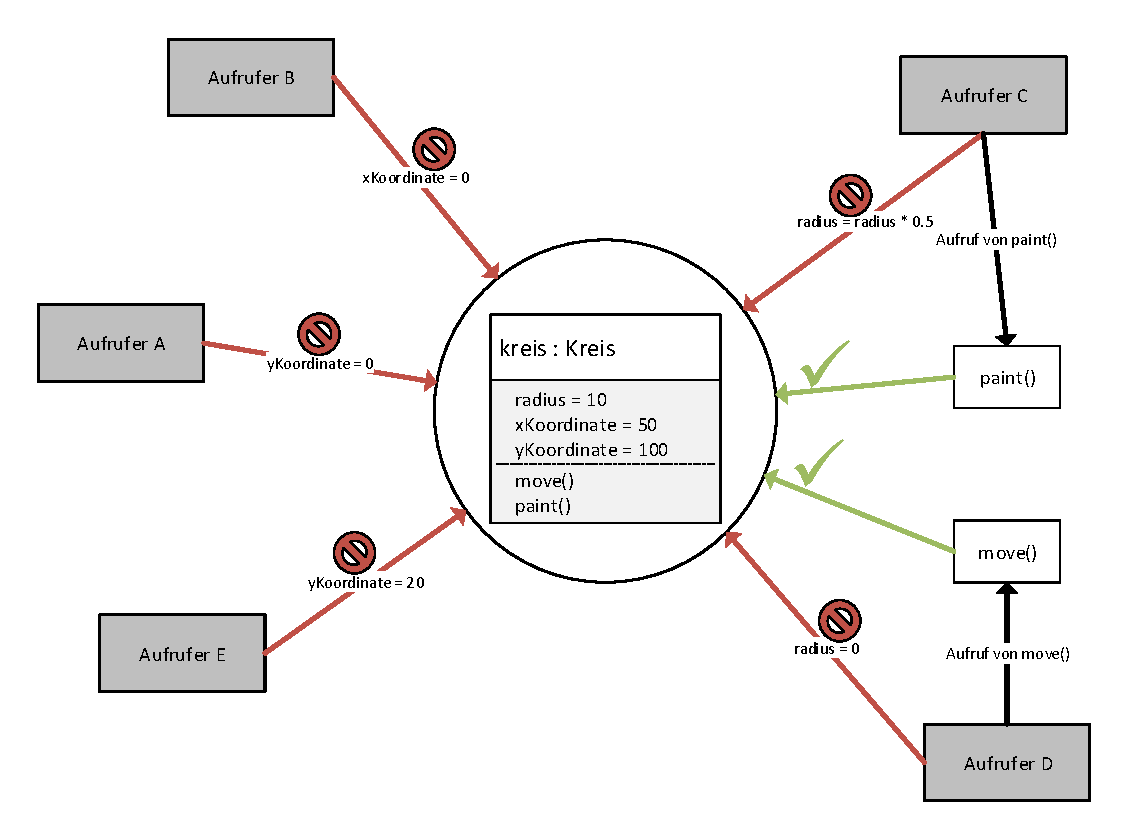
\includegraphics[height=8cm]{Images/Kapselung.pdf}
    \caption{Datenkapselung in Anlehnung an \cite[]{Lahres.2011}}
    \label{fig:Kapselung}
\end{figure}

Ein Vorteil der Datenkapselung ist laut \cite[]{Lahres.2011}, dass ein Objekt selbst für die Konsistenz seiner Daten sorgen kann. 
Von \cite[S.86f]{PoetzschHeffter.2009} wird als Vorteil der das Prinzip des \emph{Information Hiding} genannt. 
Da auf die Daten nur über eine definierte Schnittstelle zugegriffen werden kann, ist es möglich Implementierungsdetails hinter der Schnittstelle zu ändern ohne das Programmteile, die diese Klasse verwenden, angepasst werden müssen. 
Dies setzt voraus, dass die Schnittstelle gleich bleibt.

Um den Zugriff auf die Daten eines Objektes zu unterbinden oder zu ermöglichen, bietet Go die Möglichkeit die Eigenschaften eines Objektes, ähnlich der Zugriffsmodifizierer in Java, entweder \emph{Public} oder \emph{Private} zu deklarieren. 
Im Unterschied zu Java verwendet Go allerdings keine Schlüsselwörter wie \emph{Public} oder \emph{Private}.
Wird in Go der erste Buchstabe des Names eines Typs, Variable/Konstante oder Funktion klein geschrieben, ist das Element nur innerhalb des \emph{Package} sichtbar, also Private. 
Wird der erste Buchstaben des Names jedoch groß geschrieben, ist dass Element auch außerhalb des \emph{Package} sichtbar, also Public.
Das \autoref{lst:KapselungGo} zeigt ein Beispiel für diesen Mechanismus. 
In Zeile 6 wird eine Eigenschaft \emph{age} definiert die aufgrund der Kleinschreibung nicht aus dem Package \emph{animals} exportiert wird. 

\begin{listing}[H]
\caption{Datenkapselung in Go \cite[]{Kennedy.GoExport}}
\label{lst:KapselungGo}
\begin{GoCode}
package animals

type Dog struct {
    Name string
    BarkStrength int
    age int
}
\end{GoCode}
\end{listing}

Eine Anwendung der struct \emph{Dog} ist in \autoref{lst:KapselungGo2} zu sehen.
Nachdem in Zeile 5 das Package \emph{animals} importiert wurde, kann die struct \emph{Dog} verwendet werden.
Da die Eigenschaft \emph{age} nicht aus dem Package \emph{animals} exportiert wird, gibt der Compiler die Fehlermeldung aus Zeile 17 aus. 

\begin{listing}[H]
\caption{Datenkapselung in Go \cite[]{Kennedy.GoExport}}
\label{lst:KapselungGo2}
\begin{GoCode}
package main

import (
    "fmt"
    "animals"
)

func main() {
    dog := animals.Dog{
        Name:         "Chole",
        BarkStrength: 10,
        age:          5,
    }
    fmt.Printf("Counter: %#v\n", dog)
}
//Compiler-Fehler: 
//./main.go:14: unknown animal.Dog field ‘age’ in struct literal
\end{GoCode}
\end{listing}

Eine Möglichkeit die Eigenschaft \emph{age} zugänglich zu machen, ist den Zugriff über eine Get-Funktion und Set-Funktion zu realisieren.
Hierzu wurde im \autoref{lst:KapselungGo3} jeweils eine Funktion für den lesenden und schreibenden Zugriff auf die Eigenschaft \emph{age} implementiert. 
Die beiden Funktionsnamen setzen sich aus dem Namen der jeweiligen Eigenschaft, hier \emph{Age} und einem Prefix, \emph{Get} oder \emph{Set}, zusammen.
Es ist zu beachten, dass die Namen der beiden Funktionen (\emph{SetAge} und \emph{GetAge}) mit einem Großbuchstaben beginnen, da diese sonst nicht exportiert werden. 
Um den Ansatz der Datenkapselung konsequent zu verfolgen, sollten im \autoref{lst:KapselungGo3} auch die Eigenschaften \emph{Name} und \emph{BarkStrength} auf diese Art implementiert werden.   

\begin{listing}[H]
\caption{Datenkapselung in Go}
\label{lst:KapselungGo3}
\begin{GoCode}
package animals

type Dog struct {
    Name string
    BarkStrength int
    age int
}

func (d *Dog) SetAge(age int) {
    d.age = age
}

func (d *Dog) GetAge() int {
    return d.age
}
\end{GoCode}
\end{listing}

Auch Swift bietet die Möglichkeit über bietet Möglichkeiten zur Zugriffskontrolle. 
Die Zugriffs-Level sind relativ zu der Quellcodedatei und dem Modul in dem die Entität definiert wurde \cite[S.394]{Apple.2017}.
Laut der offiziellen Dokumentation \cite[S.394]{Apple.2017} bietet Swift die folgenden fünf Zugriffs-Level

\begin{itemize}
    \item Open access
    \item Public access
    \item Internal access
    \item File-private access
    \item Private access
\end{itemize}

Eine Entität, die als \textit{open} oder \textit{public} deklariert wurde, kann aus jeder Quellcodedatei im gleichen Modul verwendet werden. 
Ebenso kann jede Quellcodedatei, welche das Modul importiert in dem die Entität definiert wurde, auf die Entität zugreifen. 
Das Schlüsselwort \textit{open} greift nur bei Klassen und deren Eigenschaften.
Eine Klasse die als \textit{open} deklariert wurde, kann auch außerhalb ihres eigenen Moduls, vererbt werden, wenn das zugehörie Modul importiert wurde.
Dies unterscheidet das \textit{open}-Zugriffslevel von dem \textit{public}-Zugriffslevel.
Wird eine Entität als \textit{internal} definiert, ist diese lediglich in Quellcodedateien des eigenen Moduls verfügbar. 
Das Zugriffslevel \textit{fileprivate} schränkt den Zugriff auf die eigene Quellcodedatei ein.
Das restriktivste Zugriffslevel, \textit{private}, schränkt den Zugriff auf die umschließende Deklaration, beispielsweise eine Klasse, ein.
Ist kein Zugriffslevel definiert, verwendet der Compiler das \textit{internal}-Zugriffslevel.

\begin{listing}
\caption{Zugriffslevel in Swift \cite[S.396]{Apple.2017}}
\label{lst:ZugriffslevelSwift}
\begin{SwiftCode}
public class SomePublicClass {}
internal class SomeInternalClass {}
fileprivate class SomeFilePrivateClass {}
private class SomePrivateClass {}

public var somePublicVariable = 0
internal let someInternalConstant = 0
fileprivate func someFilePrivateFunction() {}
private func somePrivateFunction() {}
\end{SwiftCode}
\end{listing}

Neben der Möglichkeit den Zugriff zu beschränken, bietet Swift die Möglichkeit Getter/Setter zu verwenden.
autoref{lst:DatenkapselungSwfit} zeigt ein Beispiel für Datenkapselung in Swift. 
Das Beispiel wurde analog zu dem \autoref{lst:KapselungGo3} in Go implementiert.

\begin{listing}
\caption{Datenkapselung in Swift}
\label{lst:DatenkapselungSwfit}
\begin{SwiftCode}
class Dog {
    var Name : String = ""
    var BarkStrength : Int = 0
	
    private var _age : Int = 0
    public var Age : Int {
        get{return _age}
        set{_age = newValue}
    }
}
\end{SwiftCode}
\end{listing}

Die verschiedenen Zugriffslevel in Swift ermöglichen es den Zugriff auf Entitäten viel feiner zu steuern als in Go.
Die Möglichkeit von Go, Entitäten als \textit{private} zu deklarieren (Kleinschreibung des Namens), ist in Swift mit dem Zugriffslevel \textit{iternal access} vergleichbar (Schlüsselwort \textit{interal}). 
Wird in Go eine Entität als \textit{public} deklariert (Großschreibung des Namens), ist dies mit dem Zugriffslevel \textit{public access} (Schlüsselwort \textit{public}) in Swift zu vergleichen.
Der Einsatz von Getter/Setter-Methoden in Swift ermöglicht dem Programmierer eine einfachere Schreibweise von Zuweisungen. 
In \autoref{lst:GetterSetterSWift} ist die Verwendung der Klasse aus \autoref{lst:DatenkapselungSwfit} zu sehen. 
der Variable \textit{aDog} wird eine neue Instanz der Klasse \textit{Dog} zugewiesen.
Anschließend wird der Instanzvariablen \textit{Age} der Wert 2 zugewiesen.

\begin{listing}
\caption{Einsatz von Getter/Setter in Swift}
\label{lst:GetterSetterSWift}
\begin{SwiftCode}
var aDog = Dog()

aDog.Age = 2

\end{SwiftCode}
\end{listing}

In Go sieht die Verwendung von Getter/Setter-Methoden aus, wie in \autoref{lst:GetterSetterGo} abgebildet.
Da Go keine expliziten Getter/Setter-Methoden unterstützt, ist das Vorgehen aus \autoref{lst:KapselungGo3} und \autoref{lst:GetterSetterGo} an die Konvention gebunden, dass Instantzvariablen \textit{private} sind und der Zugriff auf die Werte der Instanzvariablen rein über eigens implementierte Getter/Setter-Methoden erfolgt.
Um das Konzept der Datenkapselung in Go zu verfolgen, muss diese Konvention eingehalten werden.
Swift erleichtert es dem Entwickler, dieses Konzept zu verfolgen.

\begin{listing}
\caption{Einsatz von Getter/Setter in Go}
\label{lst:GetterSetterGo}
\begin{GoCode}
var Dog = new(animals.Dog)

Dog.SetAge(2)
\end{GoCode}
\end{listing}

\section{Polymorphie}
Neben Vererbung und Datenkapselung ist Polymorphie ein Grundelement der Objektorientierten Programmierung.
\cite[]{Lahres.2011} versteht unter Polymorphie in der Objektorientierten Programmierung, dass verschiedene Objekte bei Aufruf derselben Operation unterschiedliches Verhalten zeigen können. 
In \autoref{fig:Polymorphie} wird ein praktisches Beispiel für Polymorphie aus dem Alltag gezeigt. 

\begin{figure}[H]
    \centering
    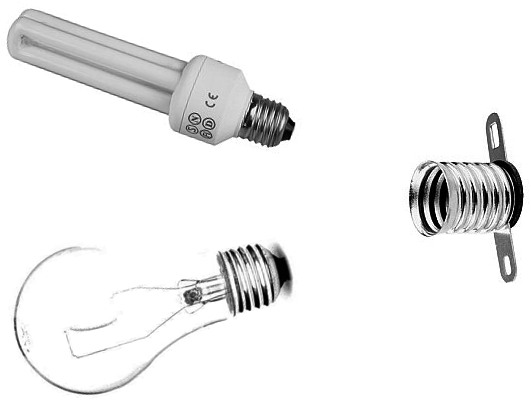
\includegraphics[height=5cm]{Images/Polymorphie}
    \caption{Beispiel für Polymorphie \cite[]{Lahres.2011}}
    \label{fig:Polymorphie}
\end{figure}

Polymorphie wird von \cite[]{Lahres.2011} mit ,,Vielgestaltigkeit'' übersetzt. Das Beispiel von \cite[]{Lahres.2011} bezieht sich auf die in \autoref{fig:Polymorphie} abgebildeten Glühbirnen und die zugehörige Fassung. 
Eine Glühbirne kann unterschiedliche Formen und Stärken haben, aber solange sie sich an die Norm für die Fassung hält, wird sie in der Fassung funktionieren. 
In Bezug auf Objektorientierung nennt \cite[]{Lahres.2011} das Beispiel ein Berechnungsverfahren gegen ein effizienteres Berechnungsverfahren zu tauschen. 
Hierzu muss nur das Berechnungsverfahren, die Glühbirne, gegen eine neue Implementierung getauscht werden und in die vorgesehen ,,Fassung'' geschraubt werden.

\begin{quote}
\enquote{An den richtigen Punkten eingesetzt, kann die Nutzung der Polymorphie dadurch zu wesentlich flexibleren Programmen führen. Sie steigert damit die Wartbarkeit und Änderbarkeit unserer Software.}
\cite[]{Lahres.2011}
\end{quote}

An dieser Stelle soll der Einsatz von Polymorphie in Go und Swift untersucht werden. 
Nach Ansicht von \cite[]{WilliamKennedy.2013} ist Vererbung ohne Polymorphie nutzlos, und die Art der Implementierung von Interfaces in Go macht Vererbung überflüssig. 
Als Grundlage dient das \autoref{lst:VererbungGo}. 

\begin{listing}[H]
\caption{Polymorphie in Go in Anlehung an \cite[]{WilliamKennedy.2013}}
\label{lst:PolymorhpieGo}
\begin{GoCode}
package main

import (
    "fmt"
)

type Animal struct {
    Name string
    mean bool
}

type AnimalSounder interface {
    MakeNoise()
}

type Dog struct {
    Animal
    BarkStrength int
}

type Cat struct {
    Basics Animal
    MeowStrength int
}

func (animal *Animal) PerformNoise(strength int, sound string) {
    if animal.mean == true {
        strength = strength * 5
    }

    for voice := 0; voice < strength; voice++ {
        fmt.Printf("%s ", sound)
    }

    fmt.Println("")
}

func (dog *Dog) MakeNoise() {
    dog.PerformNoise(dog.BarkStrength, "BARK")
}

func (cat *Cat) MakeNoise() {
    cat.Basics.PerformNoise(cat.MeowStrength, "MEOW")
}

func MakeSomeNoise(animalSounder AnimalSounder) {
    animalSounder.MakeNoise()
}
\end{GoCode}
\end{listing}

Im Unterschied zu \autoref{lst:VererbungGo} wurde in \autoref{lst:PolymorhpieGo} den Objekten ein Vehalten in Form von Methoden gegeben.
Im Interface \emph{AnimalSounder} ist eine Funktion \emph{MakeNoise()} definiert. 
Dieses Interface wird von \emph{Dog} (Zeile 28 - 39) und \emph{Cat} (Zeile 42 - 44) implementiert. 
Sobald in Go ein Type ein Interface implementiert, repräsentiert dies das Interface. 
Die Implementierungen des Interfaces rufen wiederum die auf dem Type \emph{Animal} implementierte Funktion \emph{PerformNoise} auf.
Der Funktion \emph{MakeSomeNoise} wird ein Übergabeparameter vom Typ des Intefaces \emph{Animalsounder} übergeben. 
Das Interface \emph{AnimalSounder} und die Funktion \emph{MakeSomeNoise} sorgen für das polymorphe Verhalten \cite[]{WilliamKennedy.2013}.  

Das \autoref{lst:PolymorhpieGo2} zeigt die Verwendung der Typen \emph{Dog} und \emph{Cat}.
Dazu wird jeweils eine Instanz vom Type \emph{Dog} und vom Type \emph{Cat} erstellt. 
Anschließend wird die Funktion \emph{MakeSomeNoise} jeweils mit den erzeugten Instanzen von \emph{Cat} und \emph{Dog} aufgerufen. 
Dies ist möglich, da \emph{Cat} und \emph{Dog} das Interface \emph{AnimalSounder} implementieren. 

\begin{listing}[H]
\caption{Polymorphie in Go in Anlehung an \cite[]{WilliamKennedy.2013}}
\label{lst:PolymorhpieGo2}
\begin{GoCode}
package main

func main() {
    myDog := &Dog{
        Animal{
            "Rover", // Name
            false,   // mean
        },
        2, // BarkStrength
    }

    myCat := &Cat{
        Basics: Animal{
            Name: "Julius",
            mean: true,
        },
        MeowStrength: 3,
    }

    MakeSomeNoise(myDog)
    MakeSomeNoise(myCat)
}
//Ausgabe:
//BARK BARK
//MEOW MEOW MEOW MEOW MEOW MEOW MEOW MEOW MEOW MEOW MEOW 
//MEOW MEOW MEOW MEOW
\end{GoCode}
\end{listing}

Um in Swift Polymorphie zu implementieren, werden \textit{protocols} eingesetzt.
\textit{Protocols} sind ähnlich zu \textit{Interfaces} aus anderen Programmiersprachen wie Java und Go.
Von Apple werden \textit{protocols} wie folgt definiert.

\begin{quote}
\enquote{A protocol defines a blueprint of methods, properties, and other requirements that suit a particular
task or piece of functionality. The protocol can then be adopted by a class, structure, or enumeration
to provide an actual implementation of those requirements. Any type that satisfies the requirements of
a protocol is said to conform to that protocol.} \cite[S.341]{Apple.2017}
\end{quote}

In \autoref{lst:PolymorphieSwift1} ist die Swift-Implementierung von \autoref{lst:PolymorhpieGo} abgebildet.
Ähnlich einer Klasse kann ein \textit{Protocol} in Swift Eigenschaften und Methoden haben. 
In Zeile 17 - 19 wird das Protocol \textit{AnimalSounder} definiert. 
Das Protocol \textit{AnimalSounder} hat nur eine Methode \textit{MakeNoise()}. 
Die Methode \textit{MakeNoise()} wird lediglich mit ihrer Signatur definiert. 
Es wird keine Methodenkörper definiert. 
Die Implementierung der Methode \textit{MakeNoise()} muss in den Klassen \textit{Dog} und \textit{Cat} geschehen.
In Zeile 1 - 15 wird die Basisklasse \textit{Animal} definiert. 
Die Methode \textit{PerformNoise} erwartet die beiden Übergabeparameter \textit{strength} und \textit{sound}.
Die Klassen \textit{Dog} und \textit{Cat} erben von der Basisklasse \textit{Animal}.
Bei der Implementierung der Methode \textit{MakeNoise} in den Klassen \textit{Dog} und \textit{Cat} wird die von der Klasse \textit{Animal} geerbte Methode \textit{PerformNoise} mit den spezifischen Parametern aufgerufen.

\begin{listing}[H]
\caption{Polymorphie in Swift}
\label{lst:PolymorphieSwift1}
\begin{SwiftCode}
class Animal{
    var Name : String = ""
    var mean : Bool = false
	
    func PerformNoise(strength: Int, sound: String){
        var newStrength = strength
        if mean == true{
            newStrength = strength * 5
        }
		
        for _ in 0...newStrength{
            print(sound)
        }
    }
}

protocol AnimalSounder{
    func MakeNoise()
}

class Dog : Animal, AnimalSounder{
    var BarkStrength : Int = 0
	
    func MakeNoise() {
        PerformNoise(strength: BarkStrength, sound: "BARK")
    }
}

class Cat : Animal, AnimalSounder{
    var MeowStrength : Int = 0
	
    func MakeNoise() {
        PerformNoise(strength: MeowStrength, sound: "MEOW")
    }
}
\end{SwiftCode}
\end{listing}

\autoref{lst:PolymorphieSwift2} zeigt die Verwendung der Klassen aus \autoref{lst:PolymorphieSwift1}.
Die Beiden Objekte \textit{myDog} und \textit{myCat} werden mit den gleichen Werten initialisiert, welche auch in der Implementierung in Go in \autoref{lst:PolymorhpieGo2} verwendet werden..
In Zeile 11 und 12 wird bei beiden Objekten die Methode \textit{MakeNoise} aufgerufen, welche zu der Ausgabe in Zeile 15 - 17 führt. 

\begin{listing}[H]
\caption{Polymorphie in Swift}
\label{lst:PolymorphieSwift2}
\begin{SwiftCode}
var myDog = Dog()
myDog.Name = "Rover"
myDog.mean = false
myDog.BarkStrength = 2

var myCat = Cat()
myCat.Name = "Julius"
myCat.mean = true
myCat.MeowStrength = 3

myDog.MakeNoise()
myCat.MakeNoise()

//Ausgabe: 
//BARK BARK 
//MEOW MEOW MEOW MEOW MEOW MEOW MEOW MEOW MEOW MEOW MEOW 
//MEOW MEOW MEOW MEOW 
\end{SwiftCode}
\end{listing}

Es kann sowohl in Go als auch in Swift objektorientiert programmiert werden. 
Allerdings ist Go keine vollwertige objektorientierte Programmiersprache. 

\begin{quote}
\enquote{I consider Go to be a light object oriented programming language. Yes it does have encapsulation and type member functions but it lacks inheritance and therefore traditional polymorphism.} \cite[]{WilliamKennedy.2013}
\end{quote}

Swift hingegen kann als vollwertige objektorientierte Programmiersprache angesehen werden.

\begin{quote}
\enquote{Swift’s features allow it to be used as an object-oriented programming language. This
means that you do the majority of your work by creating and manipulating objects—
chunks of data and code that represent a thing that can perform some useful work or
store some useful data.} \cite[59]{Manning.2016}
\end{quote}

In den Codebeispielen konnten alle Anforderungen erfüllt werden.
Es muss jedoch berücksichtigt werden, das es sich hierbei um einfache Anforderungen handelt, die nicht der Realität entsprechen. 
Das Go keine Vererbung unterstützt ist im Vergleich zu Swift der größte Nachteil.
Die Art in der Objektorientierung in Swift umgesetzt ist, ist für Umsteiger von anderen objektorientierten Programmiersprachen (Java, C\#) einfacher zu erlernen und zu verstehen.
\cite[]{WilliamKennedy.2013} beschreibt die objektorientierten Fähigkeiten wie folgt.

\begin{quote}
\enquote{Go took the best parts of OOP, left out the rest and gave us a better way to write polymorphic code.} \cite[]{WilliamKennedy.2013}
\end{quote}

\section{Erweiterungen}
Mit \textit{Xtend}\cite[]{Xtend} ist eine Programmiersprache für die \textit{Java Virtual Machine} verfügbar, welche es erlaubt über \textit{Extension Methods} neue Methoden zu bestehenden Klassen hinzuzufügen, ohne diese zu verändern.

Swift kennt diese Funktionalität unter dem Namen \textit{Extensions}.
Ein Auszug aus der Swift Dokumentation \cite[S331]{Apple.2017} bietet einen Überblick über die Möglichkeiten, die Extensions in Swift bieten:

\begin{itemize}
    \item Add computed instance properties and computed type properties    
    \item Define instance methods and type methods
    \item Provide new initializers
    \item Define subscripts
    \item Define and use new nested types
    \item Make an existing type conform to a protocol
\end{itemize}

\autoref{lst:SwiftExtensions} zeigt die Anwendung von \textit{Extensions} in Swift.
Der Swift-Basisdatentyp \textit{Double} wird über die \textit{Extension} mit \textit{Properties} für Längenangaben erweitert.
Eine \textit{Extension} kann bestehende Funktionalitäten eines Objektes nicht überschreiben.
Auch \textit{Protocols} können mit \textit{Extensions} erweitert werden.

\begin{listing}
\caption{\textit{Extensions} in Swift Quelle: \cite[S.332f]{Apple.2017}}
\label{lst:SwiftExtensions}
\begin{SwiftCode}
extension Double {
    var km: Double { return self * 1_000.0 }
    var m: Double { return self }
    var cm: Double { return self / 100.0 }
    var mm: Double { return self / 1_000.0 }
    var ft: Double { return self / 3.28084 }
}

let oneInch = 25.4.mm
print("One inch is \(oneInch) meters") 
// Prints "One inch is 0.0254 meters"

let threeFeet = 3.ft
print("Three feet is \(threeFeet) meters")
// Prints "Three feet is 0.914399970739201 meters"
\end{SwiftCode}
\end{listing}

Go bietet dem Programmierer keine Möglichkeit bestehende Typen durch integrierte Sprachkonstrukte zu erweitern. 